En la siguiente sección se presenta una caracterización general de los datos capturados hasta el cierre de esta memoria con intenciones de aportar a los datos estadísticos relativos a Twitter en territorio Chileno.

Las cantidades de datos capturados son los siguientes:

\begin{table}[H]
	\centering
	\begin{tabular}{| l | c |}
		\hline
		Tipo de dato    & Nº\\ \hline
		Usuarios    & 650.000 \\ \hline
		Tweets		& 17.300.000 \\ \hline
	\end{tabular}
	\caption {Cantidad de datos capturados}
\end{table}

Características referentes a Twitter 

\begin{figure}[H]
	\centering
	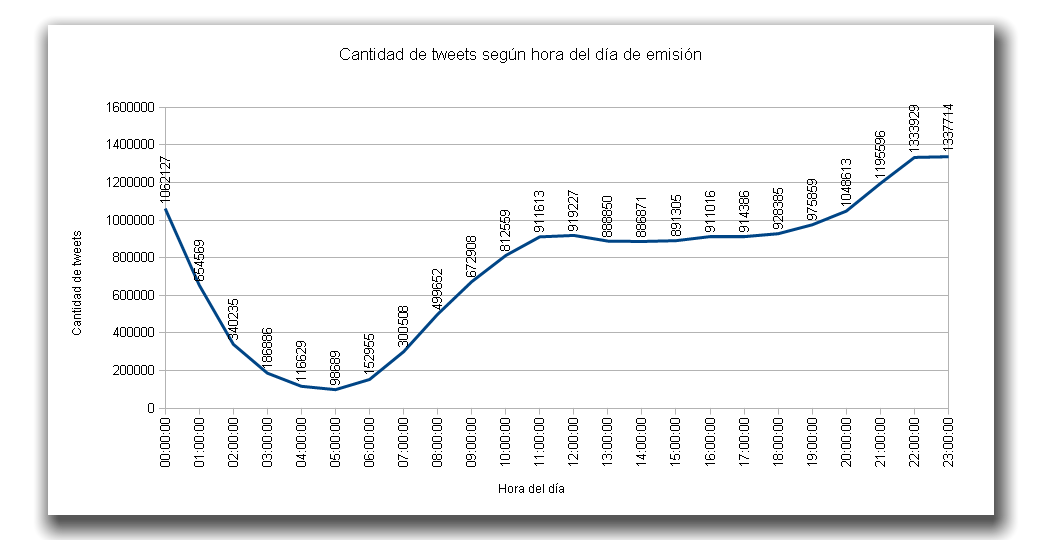
\includegraphics[width=1\textwidth]{imgs/tweets_por_hora_del_dia.png}
	\caption{Distribución de tweets por hora de emisión}
	\label{fig:tweets_por_hora}
\end{figure}

En la figura \ref{fig:tweets_por_hora} se grafica la distribución horaria de la emisión de los tweets captados. Se puede observar que las horas donde se emiten mayor cantidad de tweets comprende el periodo del día que va desde las 20:00 hrs. hasta las 23:00 hrs. mientras que el de menor emisión de tweets comprenden el periodo de horas desde las 3:00 hrs. hasta las 6:00 hrs. Se observa además que existe un periodo relativamente constante en emisión de tweets que se desarrolla desde las 11:00hrs. hasta las 20:00hrs.

La figura \ref{fig:tweets_porcentual_por_hora_por_region} representa la actividad porcentual por horas separado por región, donde se observa que existe un comportamiento similar al descrito anteriormente.

\begin{figure}[H]
	\centering
	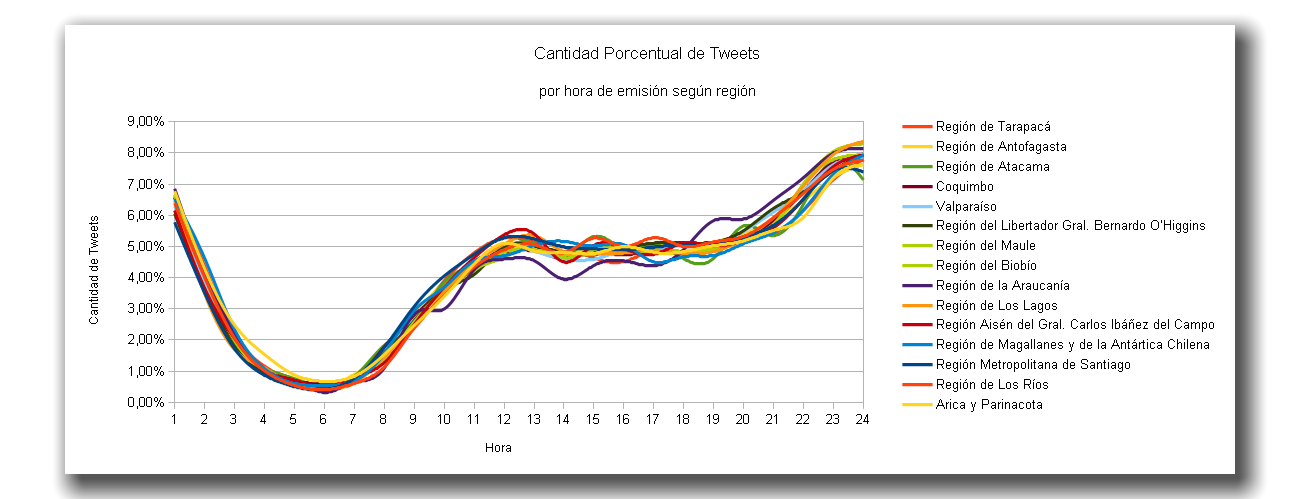
\includegraphics[width=1\textwidth]{imgs/cantidad_porcentual_de_tweets_por_hora_y_regiones.png}
	\caption{Distribución porcentual de tweets por hora de emisión según región}
	\label{fig:tweets_porcentual_por_hora_por_region}
\end{figure}



\textbf{Cantidad de re-tweets por usuario} \\

\begin{table}[H]
	\centering
	\begin{tabular}{| l | c |}
		\hline
		Medida   & Nº\\ \hline 
		Moda    & 0 \\ \hline
		Rango    & 3.424.962 \\ \hline
		Desviación Estándar    & 26.900,05 \\ \hline
		Promedio   & 711,31 \\ \hline
	\end{tabular}
	\caption {Datos cuantitativos respecto a los RT}
	\label{resumen_rt}
\end{table}

La tabla \ref{resumen_rt} nos permite observar que en cuanto al parámetro de RT el conjunto de tweets existe una variabilidad increíble respecto al promedio, lo que sugiere que existen tweets particulares con cantidades extremas de re-tweets. Tras analizar con más detalles los tweets con mayores cantidades de re-tweets se identifica una hecho insólito incluso para las macrocifras de Twitter: el tweet con más re-tweets corresponde a la famosa \emph{selfie} tomada por Ellen DeGeneres en los Oscar 2014 en conjunto a varias estrellas del cine que alcanzó el record en re-tweets con la suma de 2,5 millones de re-tweets.

\begin{figure}[H]
	\centering
	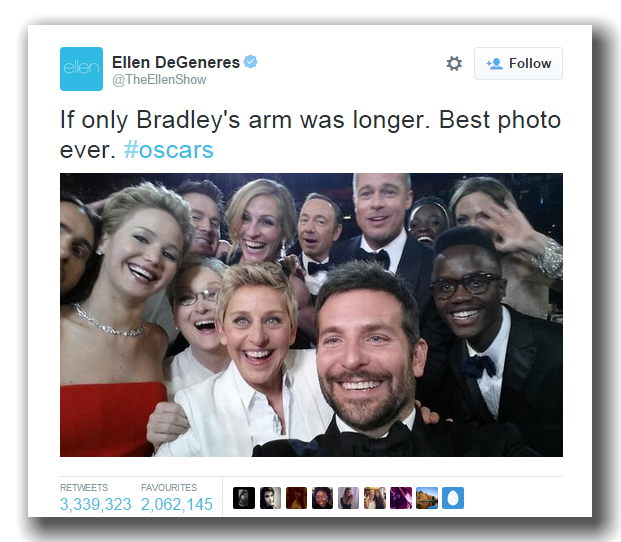
\includegraphics[width=0.5\textwidth]{imgs/ellen_selfie.png}
	\caption{Tweet que generó nuevo record del mensaje más re-tweeteado.}
	\label{fig:ellen_selfie}
\end{figure}

\textbf{Cantidad de favoritos por usuario} \\

\begin{table}[H]
	\centering
	\begin{tabular}{| l | c |}
		\hline
		Medida   				& Nº\\ \hline 
		Moda    				& 0 \\ \hline
		Rango    				& 18423 \\ \hline
		Desviación Estándar    	& 16,28 \\ \hline
		Promedio   				& 0,2602 \\ \hline
	\end{tabular}
	\caption {Datos cuantitativos respecto a los FAV}
\end{table}

De manera similar al caso de los re-tweets, la cantidad de favoritos presenta una desviación estándar más grande que el promedio captado, con la diferencia que el rango es menor. En comparativa con la tabla anterior es posible apreciar una diferencia de al menos tres ordenes de magnitud entre las medias de ambos cuantificadores.\\

\textbf{Cantidad de tweets por usuario} \\

Respecto a la cantidad de tweets se observa que el promedio son 627 tweets por cuenta de usuario como se observa en la siguiente tabla: 

\begin{table}[H]
	\centering
	\begin{tabular}{| l | c |}
		\hline
		Medida   				& Nº\\ \hline 
		Moda    				& 0 \\ \hline
		Rango    				& 718.249 \\ \hline
		Desviación Estándar    	& 4.700,45\\ \hline
		Promedio   				& 627,5728 \\ \hline
	\end{tabular}
	\caption {Cantidad de tweets por usuario}
	\label{resumen_tweets}
\end{table}
\textbf{Cantidad de Seguidores por usuario} \\

\begin{table}[H]
	\centering
	\begin{tabular}{| l | c |}
		\hline
		Medida   				& Nº\\ \hline 
		Moda    				&  1 \\ \hline
		Rango    				& 5.372.178\\ \hline
		Desviación Estándar    	& 16.504,96 \\ \hline
		Promedio   				& 427,64 \\ \hline
	\end{tabular}
	\caption {Cantidad de seguidores por usuario}
	\label{table:followers_por_usuario}
\end{table}

\textbf{Cantidad de Amigos por usuario} \\

\begin{table}[H]
	\centering
	\begin{tabular}{| l | c |}
		\hline
		Medida   				& Nº\\ \hline 
		Moda    				& 40\\ \hline
		Rango    				& 1.393.022\\ \hline
		Desviación Estándar    	& 5.283,16 \\ \hline
		Promedio   				& 364,50\\ \hline
	\end{tabular}
	\caption {Cantidad de amigos por usuario}
	\label{table:friends_por_usuario}
\end{table}

Tras comparar las tablas \ref{table:followers_por_usuario} y la tabla \ref{table:friends_por_usuario} se observa que existe una diferencia muy ajustada en los promedios obtenidos, pero que el valor máximo es superior en el caso de la cantidad de seguidores que en la cantidad de amigos de los usuarios. 

Utilizando las clasificaciones para usuarios realizadas en \cite{conf/cikm/UysalC11} en Chile su distribución es la siguiente:

\begin{table}[H]
	\centering
	\begin{tabular}{| l | c |}
		\hline
		Nombre Categoría  		& Nº\\ \hline 
		Élite Global   			& 784 \\ \hline 
		Élite Local   				& 1.611\\ \hline
		Usuario Corriente			& 624.564\\ \hline
	\end{tabular}
	\caption {Cantidad de usuarios según clasificación realizada en \cite{conf/cikm/UysalC11}}
	\label{table:cantidad_usuarios_por_clasificacion}
\end{table}

Cómo dato adicional a la tabla \ref{table:cantidad_usuarios_por_clasificacion} existen 37.808 que teniendo menos de 1000 followers no cumplen con el criterio de tener menos de 1000 amigos.\\

\textbf{Posicionamiento geográfico de los usuarios}\\

Respecto al posicionamiento de los usuarios con el método revisado en \ref{sec:geo} se obtuvo la siguiente distribución por regiones:

%revisar pagina 20 seccion 4.2.5

\begin{table}[H]
	\centering
	\begin{tabular}{| p{5.5cm} | c | c | c | c |}
		\hline
			\multirow{2}{*}{Región} & \multicolumn{2}{c|}{Usuarios Twitter} & \multicolumn{2}{c|}{Población real} \\ \cline{2-5}
			& Usuarios (M) & Porcentaje & Personas (M) & Porcentaje \\ \hline
			Región de Arica y Parinacota & 1,914 & 1,68 & 185,0 & 1,1 \\ \hline 
			Región de Tarapacá & 4,477 & 3,93 & 314,5 & 1,8 \\ \hline 
			Región de Antofagasta & 6,005 & 5,27 & 575,3 & 3,4 \\ \hline 
			Región de Atacama & 0,974 & 0,85 & 280,5 & 1,6 \\ \hline 
			Región de Coquimbo & 4,411 & 3,87 & 718,7 & 4,2 \\ \hline 
			Región de Valparaíso & 7,111 & 6,24 & 1.759,2 & 10,3 \\ \hline
			Región de O’Higgins & 4,756 & 4,17 & 883,4 & 5,2 \\ \hline 
			Región del Maule & 6,183 & 5,42 & 1.007,8 & 5,9 \\ \hline 
			Región del Biobío & 16,862 & 14,79 & 2.036,4 & 11,9\\ \hline 
			Región de la Araucanía & 0,825 & 0,72 & 970,4 & 5,7 \\ \hline 
			Región de Los Ríos & 2,245 & 1,97 & 379,7 & 2,2 \\ \hline 
			Región de Los Lagos & 4,891 & 4,29 & 836,3 & 4,9 \\ \hline
			Región de Aisén & 0,565 & 0,5 & 104,8 & 0,6 \\ \hline
			Región Magallanes y la Antártica & 1,298 & 1,14 & 158,7 & 0,9 \\ \hline  
			Región Metropolitana de Santiago & 51,499 & 45,17 & 6.883,6 & 40,3\\ \hline 
			Total & 114.016 & 100 & 17.094,3 & 100\\ \hline 
	\end{tabular}
	\caption {Distribución de los usuarios por regiones}
	\label{table:cantidad_usuarios_por_region}
	
\end{table}

En esta tabla es posible observar la concentración de usuarios existente en torno a la región metropolitana con el 45\% de los usuarios totales del país, 5 puntos porcentuales menos con respecto a la población real de Chile. Lo anterior no refleja otra cosa que la concentración del país también se ve reflejada por la cantidad de usuarios de Twitter en Chile.
